\documentclass[12pt]{article}
\usepackage[english]{babel}
\usepackage{natbib}
\usepackage{url}
\usepackage[utf8x]{inputenc}
\usepackage{amsmath}
\usepackage{graphicx}
\graphicspath{{../docs/img/}}
\usepackage{parskip}
\usepackage{fancyhdr}
\usepackage{vmargin}
\usepackage{xcolor}
\usepackage{booktabs}
\usepackage{float}
\usepackage{pgfplots}
\usepackage{tikz}
\pgfplotsset{width=10cm,compat=1.9}

\setmarginsrb{3 cm}{2.5 cm}{3 cm}{2.5 cm}{1 cm}{1.5 cm}{1 cm}{1.5 cm}

\title{Sprint 2 Backlog}								% Title
\author{Thierry's Minions}								% Author
\date{12 Sept 2015}											% Date

\makeatletter
\let\thetitle\@title
\let\theauthor\@author
\let\thedate\@date
\makeatother

\pagestyle{fancy}
\fancyhf{}
\rhead{\theauthor}
\lhead{\thetitle}
\cfoot{\thepage}

\newcommand*{\userstory}[5][.25em]{
%  \begin{tabular*}{\maincolumnwidth}{l@{\extracolsep{\fill}}r}%
%    {\bfseries #2} & {\bfseries #4}\\%
%    {#3}\\%
%  \end{tabular*}%
%  \ifx&#5&%
%  \else{\\%
%    \begin{minipage}{\maincolumnwidth}%
%      #5%
%    \end{minipage}}\fi%
%  \par\addvspace{#1}
\textbf{#1} 
  }

\newcommand{\roundpic}[4][]{
  \tikz\node [circle, minimum width = #2,
    path picture = {
      \node [#1] at (path picture bounding box.center) {
        \includegraphics[width=#3]{#4}};
    }] {};}

\begin{document}

%%%%%%%%%%%%%%%%%%%%%%%%%%%%%%%%%%%%%%%%%%%%%%%%%%%%%%%%%%%%%%%%%%%%%%%%%%%%%%%%%%%%%%%%%

\begin{titlepage}
	\centering
    \vspace*{0.5 cm}
\roundpic[]{9cm}{9cm}{leader.jpg}

    \textsc{\LARGE Thierry's Minions/Team25\\[0.5em] Deliverable 3}\\[2.0 cm]	
	\textsc{\Large CSCC01 Fall 2018}\\[0.5 cm]				% Course Code
	\rule{\linewidth}{0.2 mm} \\[0.4 cm]
	{ \huge \bfseries \thetitle}\\
	\rule{\linewidth}{0.2 mm} \\[1.5 cm]
	
	\begin{minipage}{0.4\textwidth}
		\begin{flushleft} \large
			\emph{Submitted To:}\\
			Saba Kiaei\\
            Teaching Assistant\\
            Computer Science Department\\
			\end{flushleft}
			\end{minipage}~
			\begin{minipage}{0.4\textwidth}
            
			\begin{flushright} \large
			\emph{Submitted By :} \\
			Rishabh Kaant Sharma\\
            Joseph Sokolon\\
            Balaji Badu\\
            Jayden Arquelada\\
            Edgar Sarkisian\\
		\end{flushright}
        
	\end{minipage}\\[2 cm]
	
	
    
    
    
    
	
\end{titlepage}

%%%%%%%%%%%%%%%%%%%%%%%%%%%%%%%%%%%%%%%%%%%%%%%%%%%%%%%%%%%%%%%%%%%%%%%%%%%%%%%%%%%%%%%%%

\textcolor{black}{\tableofcontents}
\pagebreak

%%%%%%%%%%%%%%%%%%%%%%%%%%%%%%%%%%%%%%%%%%%%%%%%%%%%%%%%%%%%%%%%%%%%%%%%%%%%%%%%%%%%%%%%%

\section{Sprint Tasks}

\subsection{Task 1E: Integrate Login UI and Controller}
\begin{itemize}%
\item Story Points: 2
\item This task has a dependency on task 1C, 1D
\item Integrate the login controller with the UI
\item The login request should be sent when button is clicked on UI
\item The UI should reflect whether the login operation was successful
\end{itemize}

\subsection{Task 1F: Test entire flow}
\begin{itemize}%
\item Story Points: 1
\item This task has a dependency on all previous task in story 
\item Test the entire workflow of login (Client + Server)
\item Fix any errors 
\end{itemize}

\subsection{Task 2A: Create UI Screen for Data Upload}
\begin{itemize}%
\item Story Points: 5
\item Create a JavaFX Screen that allows you to select a document from filesystem
\item Display document selected
\item Add dropdown to specify which template type it is
\item Add button which is labed "Upload" 
\end{itemize}

\subsection{Task 2B: Parse Excel file into Json}
\begin{itemize}%
\item Story Points: 5
\item Parse Excel file into JSON Client side 
\item Use Apache POI for parsing
\item Display popup window of error occured while parsing 
\end{itemize}

\subsection{Task 2C: Send JSON to server}
\begin{itemize}%
\item Story Points: 2
\item When Upload button is clicked send the JSON object of the parsed file to the server
\item Send to server using a HTTP POST Request
\end{itemize}

\subsection{Task 2D: Switch Database to MongoDB from SQL}
\begin{itemize}%
\item Story Points: 2
\item Team decided it would be better for project if we use a NoSQL database
\item Switch existing database to MongoDB from SQL
\item Use Mongo Atlas for hosting
\item Update methods and connection in database.js
\end{itemize}

\subsection{Task 2E: Save JSON sent from client in database}
\begin{itemize}%
\item Story Points: 8
\item This task has a dependency on task 2D
\item Create new endpoint on server to recieve JSON data for parsed file from client
\item Upload endpoint will be HTTP POST request to: /reports/new-report
\item Save JSON sent in upload request to database
\end{itemize}

\subsection{Task 2F: Integrate and test entire flow}
\begin{itemize}%
\item Story Points: 5
\item This task has a dependency on all previous task in story 
\item Integrate parts and fix any errors 
\item Test the entire workflow of uploading data (Client + Server)

\end{itemize}

\newpage
\section{Sprint Plan}
\color{red}IMPORTANT NOTE: The team did not sprint from  October 13th - October 19th due to assignments due after reading week
\color{black}

\textbf{Sprint 2 : October 20th - October 26th (Saturday - Friday)}
\begin{table}[H]
\begin{tabular}{@{}c|c|c|c|ccccccc@{}}
\toprule
Story & Task & Dependency & \begin{tabular}[c]{@{}c@{}}Story\\ Points\end{tabular} & \begin{tabular}[c]{@{}c@{}}Day\\ 1\end{tabular} & \begin{tabular}[c]{@{}c@{}}Day\\ 2\end{tabular} & \begin{tabular}[c]{@{}c@{}}Day \\ 3\end{tabular} & \begin{tabular}[c]{@{}c@{}}Day \\ 4\end{tabular} & \begin{tabular}[c]{@{}c@{}}Day \\ 5\end{tabular} & \begin{tabular}[c]{@{}c@{}}Day \\ 6\end{tabular} & \begin{tabular}[c]{@{}c@{}}Day \\ 7\end{tabular} \\ \midrule
1     & E    &            & 2                                                      & BB:2                                            &                                                 &                                                  &                                                  &                                                  &                                                  &                                                  \\
1     & F    & E          & 1                                                      &                                                 & JS:1                                            &                                              &                                                  &                                                  &                                                  &                                                  \\
2     & A    &            & 5                                                      & JA:4                                            &                                                 & JA:1                                             &                                                  &                                                  &                                                  &                                                  \\
2     & B    &            & 5                                                      &                                                 & ES:3                                            & ES:2                                             &                                                  &                                                  &                                                  &                                                  \\
2     & C    &            & 2                                                      &                                                 &                                                 &                                                  &                                                  &                                                  & BB:2                                             &                                                  \\
2     & D    &            & 2                                                      & JS:2                                            &                                                 &                                                  &                                                  &                                                  &                                                  &                                                  \\ 
2     & E    & D          & 8                                                      &                                                 &                                                 &                                                  &                                                  &  RS:4                                            &  RS:4                                            &                                                  \\ 
2     & F    & ALL        & 5                                                      &                                                 &                                                 &                                                  &                                                  &                                                  &                                                  & JS:5                                             \\ \bottomrule
\end{tabular}
\end{table}

\begin{itemize}%
\item Estimated story points team can complete: 30
\item Balaji will complete task 1E by end of day 1.
\item Joey will complete task 1F, and release feature by end of day 2.
\item Jayden will complete task 2A by end of day 3.
\item Edgar will complete task 2B by end of day 3.
\item Balaji will complete task 2C by end of day 6.
\item Joey will complete task 2D by end of day 1.
\item Rishabh will complete task 2E by end of day 6.
\item Joey will complete task 2F, and release feature by end of day 7.
\item The team believes they can complete User Story 1 \& 2 by end of the day 7. 
\end{itemize}

\newpage

\section{Sprint Report}

\textbf{Sprint 2 : October 20th - October 26th (Saturday - Friday)}

\begin{table}[H]
\begin{tabular}{@{}c|c|c|c|ccccccc@{}}
\toprule
Story & Task & Dependency & \begin{tabular}[c]{@{}c@{}}Story\\ Points\end{tabular} & \begin{tabular}[c]{@{}c@{}}Day\\ 1\end{tabular} & \begin{tabular}[c]{@{}c@{}}Day\\ 2\end{tabular} & \begin{tabular}[c]{@{}c@{}}Day \\ 3\end{tabular} & \begin{tabular}[c]{@{}c@{}}Day \\ 4\end{tabular} & \begin{tabular}[c]{@{}c@{}}Day \\ 5\end{tabular} & \begin{tabular}[c]{@{}c@{}}Day \\ 6\end{tabular} & \begin{tabular}[c]{@{}c@{}}Day \\ 7\end{tabular} \\ \midrule
1     & E    &            & 2                                                      &                                                 &                                                 &                                                  &    BB:2                                          &                                                  &                                                  &                                                  \\
1     & F    & E          & 1                                                      &                                                 &                                                 &                                              &                                                  &   JS:1                                           &                                                  &                                                  \\
2     & A    &            & 5                                                      & JA:4                                            &                                                 &     							&                                                  &                                                  &                                                  &                                                  \\
2     & B    &            & 5                                                      &                                                 & ES:4                                            & ES:6                                             &                                                  &                                                  &                                                  &                                                  \\
2     & C    &            & 2                                                      &                                                 &                                                 &                                                  &                                                  &                                                  & BB:2                                             &                                                  \\
2     & D    &            & 2                                                      & JS:2                                            &                                                 &                                                  &                                                  &                                                  &                                                  &                                                  \\ 
2     & E    & D          & 8                                                      &                                                 &                                                 &                                                  &                                                  &                                                  &                                                  & RS:8                                             \\ 
2     & F    & ALL        & 5                                                      &                                                 &                                                 &                                                  &                                                  &                                                  &                                                  & JS:5                                             \\ \bottomrule
\end{tabular}
\end{table}

\begin{itemize}%
\item Actual story points burned: 30
\item Balaji didn't complete task 1E until day 4
\item Jayden finished task 2A early on day 1
\item Task 2B took Edgar 5 hours longer then expected, he still finished by day 3.
\item Rishabh started and completed task 2E on day 7.
\item The team completed user story 1 \& 2 by end of the sprint 2. 
\end{itemize}

\section{Sprint Burndown Chart}

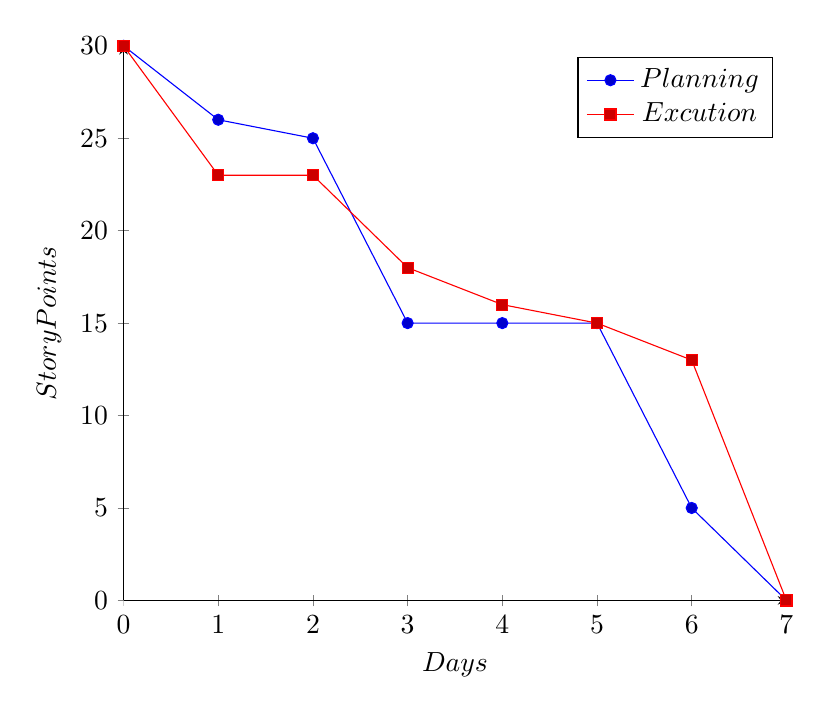
\begin{tikzpicture}
\begin{axis}[
    axis lines = left,
    xlabel = $Days$,
    ylabel = {$Story Points$},
]
\addplot coordinates {(0,30) (1,26) (2,25) (3,15) (4,15) (5,15) (6,5) (7,0)};
\addlegendentry{$Planning$}
\addplot coordinates {(0,30) (1,23) (2,23) (3,18) (4,16) (5,15) (6,13) (7,0)};
\addlegendentry{$Excution$}
\end{axis}
\end{tikzpicture}

\newpage
\bibliographystyle{plain}
\bibliography{biblist}

\end{document}